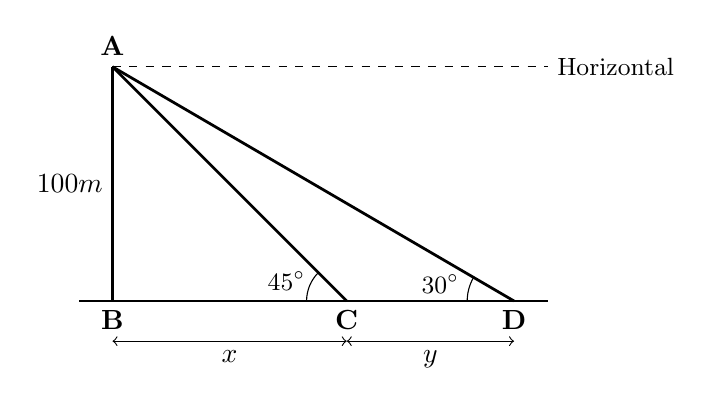
\begin{tikzpicture}[scale=0.85]
        % Horizontal ground/sea level
        \draw[thick] (-0.5,0) -- (6.5,0);
        
        % Lighthouse AB
        \draw[line width=1.2pt] (0,0) -- (0,3.5) node[above] {\textbf{A}};
        \node[below] at (0,0) {\textbf{B}};
        \node[left] at (0,1.75) {$100\text{ m}$};
        
        % Ships C and D
        \coordinate (C) at (3.5,0);
        \coordinate (D) at (6,0);
        \node[below] at (C) {\textbf{C}};
        \node[below] at (D) {\textbf{D}};
        
        % Lines of sight
        \draw[line width=1pt] (0,3.5) -- (3.5,0);
        \draw[line width=1pt] (0,3.5) -- (6,0);
        
        % Horizontal reference line at top for angles of depression
        \draw[dashed] (0,3.5) -- (6.5,3.5) node[right] {\small Horizontal};
        
        % Angles of elevation (alternate interior to angles of depression)
        \draw (2.9,0) arc (180:135:0.6);
        \node at (2.6,0.3) {\small $45^\circ$};
        
        \draw (5.3,0) arc (180:150:0.7);
        \node at (4.9,0.25) {\small $30^\circ$};
        
        % Distance labels
        \draw[<->] (0,-0.6) -- (3.5,-0.6) node[midway,below] {$x$};
        \draw[<->] (3.5,-0.6) -- (6,-0.6) node[midway,below] {$y$};
    \end{tikzpicture}
